\documentclass[13pt, a4paper, twoside]{article}z
\usepackage[utf8]{inputenc}
\usepackage{geometry}
\usepackage[czech]{babel}
\usepackage{chemformula}
\usepackage{chemfig}
\usepackage{enumitem}
\usepackage{fancyhdr}
\usepackage{float}
\usepackage{caption}
\usepackage{setspace}
\usepackage{multicol}
\geometry{legalpaper, margin=1.05in}
\pagestyle{fancy}
\lhead{\Large Šárka Doležalová, skupina 6}
\rhead{\large 10.12.2020}
\begin{document}
\begin{center}
    \Huge
    Úloha 8: Rektifikace a práce s plyny
\end{center}
\large \onehalfspacing
\section*{Zadané úlohy}
\begin{enumerate}
    \item Rektifikací rozdělte směs ethyl-acetátu a toluenu. Průběh závislosti teploty varu na čase
    vyjádřete graficky. U jednotlivých frakcí změřte jejich index lomu.
    \item  Na základě teplot varu a indexů lomu jednotlivých frakcí určete zastoupení jednotlivých
    složek ve výchozí směsi.
    \item Určete obsah uhličitanu vápenatého ve vzorku mramoru.
\end{enumerate}

\section*{Teoretický úvod}
\subsection*{Rektifikace}
Rektifikace je destilační metoda, která využívá rozdílných teplot varu dvou látek v homogenní směsi. Tím pádem látka, která má nižší teplotu varu je koncentrovanější v páře a látka s vyšší teplotou varu je koncentrovanější v kapalině.


Děj probíhá v rektifikační koloně v její horní části je odpařována látka s nižší teplotou varu. Na kolonu je dále připevněn chladič a kapalina já odtud jímaná pomocí refluxu.

\subsection*{Měření indexu lomu}
Index lomu je poměr rychlosti světla ve vakuu a v dané kapalině.

\begin{align*}
    n = \frac{c}{v}
\end{align*}


Index lomu měříme na tzv refraktometru. My užíváme refraktometr Abbeova typu. Jeho jádro se skládá ze dvou hranolů (měřící a osvětlovacího) Mezi ně se vkládá příslušná tekutina. To celé je pozorováno okulárem, abychom zjistili daný index lomu.

\subsection*{Práce s plyny}
Při různých chemických reakcích dochází k uvolňování různých plynů. Z jejich objemu můžeme spočítat ji jejich množství v původním vzorku pomocí vzorce.
\begin{align*}
    pV=nRT
\end{align*}

Kdy p jest tlak ($Pa$), V objem plynu ($m^3$), n látkové množství plynu ($mol$), R univerzální plynová konstanta  (R = 8,314 $J\cdot mol^{-1}\cdot K^{-1}$) a T je termodynamický teplota (K)
Nejjednodušeji určujeme objem plynu v eudiometru. Eudiometr je sestaven z odměrného válce naplněného uzavírací kapalinou, ponořeného vrškem ve vaně také naplněné uzavírací kapalinou. Objem jímaného plynu je roven objemu uzavírací kapaliny, která byla z válce vytlačena, odečítáme jej rovnou na stupnici válce.

\section*{Postup}
\subsection*{Rozdělení směsi ethyl-acetáty a toulenu rektifikací}
Do stojánku bylo připraveno osm popsaných zkumavek. Do 250 ml kulaté baňky byly vloženy varné kamínky a bylo nalito 100 ml směsi určené k destilaci. Baňka byla připojena ke koloně a topné hnízdo bylo posunuto tak, aby baňka dosedla. Bylo započato zahřívání a voda byla puštěna do chladiče. Kohout refluxu byl zavřený. Na koloně byla ustavána rovnováha 5 minut od doby, co se směs v baňce začala vařit. Postavení rovnováhy byly do zkumavek jímány jednotlivé frakce. Během rektifikace byla v minutových intervalech zaznamenávána teplota.
\begin{figure}[H]
    \centering
    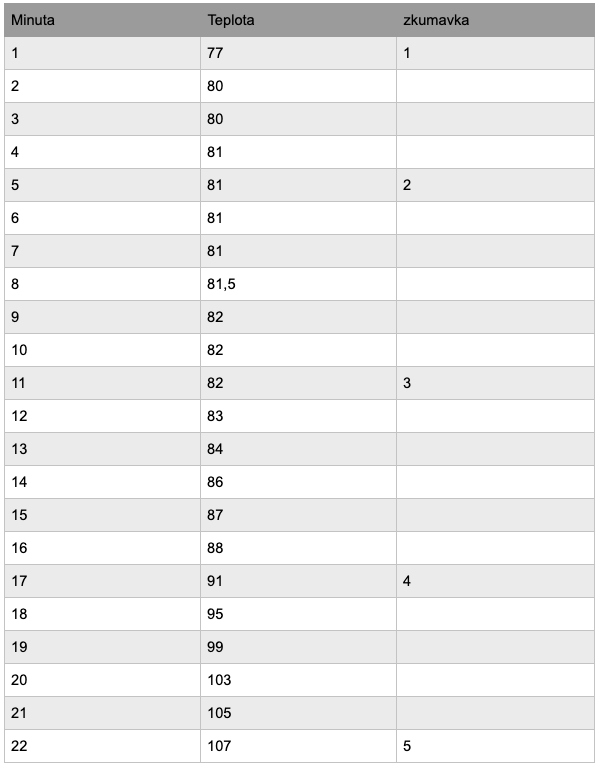
\includegraphics[width=6.5in]{uloha_8_tab_1.png}
\end{figure}
\newpage
\begin{figure}[H]
    \centering
    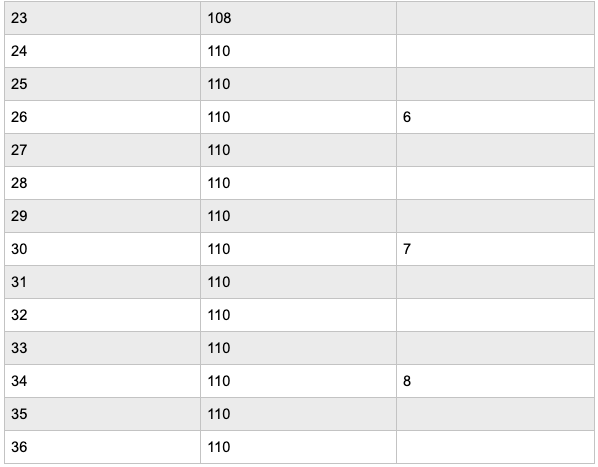
\includegraphics[width=6.5in]{uloha_8_tab_2.png}
\end{figure}

\begin{figure}[H]
    \centering
    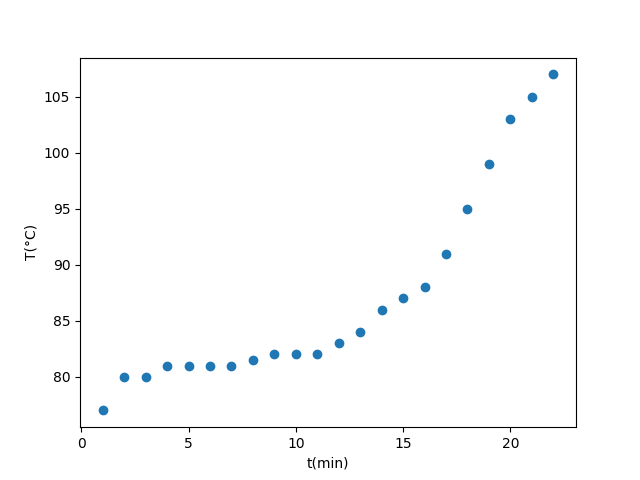
\includegraphics[width=6in]{teplota_cas.png}
\end{figure}

Po najímání 75 ml destilátu bylo vypnuto topné hnízdo, setrvačností se dojímalo posledních 5 ml.

Grafický záznam destilace – graf závislosti teploty varu směsi na čase
Na refraktometru byly změřeny indexy lomu standardu toluenu a ethyl acetátu a následně jednotlivých frakcí jednotlivých frakcí.

\begin{figure}[H]
    \centering
    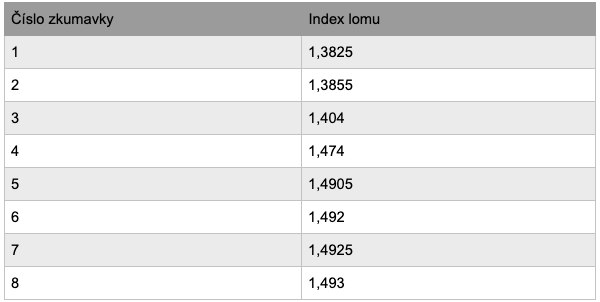
\includegraphics[width=6.5in]{uloha_8_tab_3.png}
    \caption*{Tabulka indexu lomu jednotlivých frakcí}
\end{figure}

Podle naměřených údajů bylo odhadnuto v jakém poměru byl toluen a ethyl acetát zastoupen v původním roztoku.

\subsection*{Eudiometrické stanovení obsahu $CaCO_3$ ve vzorku mramoru}
Byla sestavena eudiometrická aparatura  a bylo naváženo 1,00 g neznámého vzorku. Navážka byla opatrně vložena na dno baňky. Zátku, která uzavírala přikapávací nálevku byla nahrazena zátkou s trubičkou. Ta byla připojena k ocelové lahvi s $CO_2$ a byl otevřen kohout přikapávací nálevky. Poté byl otevřen ventil tlakové láhve. Oxid uhličitý byl mírným proudem ponechán procházet aparaturou, po 5 minutách byl přívod $CO_2$ zastaven. Eudiometr, v našem případě odměrný válec, byl naplněn vodou, dále byla pod spodní okraj zasunuta zaváděcí trubička.


Do překapávací nálevky bylo nalito 10 ml koncentrované HCl. Aparatura byla uzavřena zátkou. Byl otevřen kohout a kyselina nakapala na neznámý vzorek. Při reakci se uvolňovalo CO2, který bylo zachytáváno do odměrného válce. Bylo odečteno jeho množství. Byla zapsána teplota vody ($t_{H_2O}$ = 28 $^{\circ}C$ = 301,15 $K$) a tlak v laboratoři (p = 765 mb = 76,5 kPa = 76500 Pa).Podle rovnice $CaCO_3 + 2HCl \to CaCl_2 + CO_2 + H_2O$, můžeme vidět, že látkové množství je CO2 stejné jako $CaCO_3$. Byla vypočítána hmotnost $CaCO_3$.

\section*{Výpočty}
\subsection*{Hmotnost uhličitanu vápenatého}
$t_{H_2O}=28^{\circ}C = 301.15\: K$\\
$p = 765\: mb = 76500\:Pa$\\
$V_{CO_2}=196ml = 0.000196\:m^3$\\
$p_{aq}=3.778\:kPa=3778\:Pa$\\
$M_{CaCO_3} = 100.09 \: g\cdot mol^{-1}$\\
$R = 8.314\: J\cdot mol^{-1}\cdot K^{-1}$

\begin{align*}
    m_{CaCO_3} &= M\cdot\frac{(p-p_{aq})\cdot V}{R\cdot T}\\
    m_{CaCO_3} &= 0.5698 \: g
\end{align*}

\subsection*{Hmotnostní zlomek uhličitanu vápenatého}
$m_{CaCO_3}=0.5698\:g$\\
$m = 1\: g$

\begin{align*}
    w_{CaCO_3} &= \frac{m_{CaCO_3}}{m}\\
    w_{CaCO_3} &= 56.98\%
\end{align*}

\section*{Závěr}
Rektifikací byl zjištěn poměr směsi ethylacetát:toluen 3:7. V druhé části úlohy byl pomocí eudiometrického stanovení spočítán obsah CaCO3 ve vzorku mramoru spočítán na 56,98\%.



\end{document}